\chapter{Conclusions}
\label{cha:conclusions}

This dissertation investigated the design, implementation, and evaluation of the 2011 UH Kukui Cup challenge. This chapter summarizes the results of the research, the contributions of the research, and possible future directions.


\section{Research Summary}

In an effort to foster energy conservation and increase energy literacy in students living in campus residence halls, we designed the Kukui Cup challenge. Based on a review of the literature, the Kukui Cup challenge combines a variety of elements into an overall game experience, including: real-time energy feedback, energy conservation goals, activities, commitments, real-world events, competition between teams, and prizes.

We designed a software system called Makahiki to provide the online portion of the Kukui Cup challenge that players experience through the challenge website. We installed 40 smart meters to monitor the electricity use of each pair of floors in the four Hale Aloha tower residence halls, with the data stored in the WattDepot system.

In October 2011, we ran the 2011 UH Kukui Cup challenge for the over 1000 residents of the Hale Aloha towers over three weeks. To evaluate the Kukui Cup challenge, I conducted three experiments on: challenge participation, energy literacy, and energy use.

Many residents (37\%) participated in the challenge, as measured by points earned and actions completed through the challenge website. Participation rates for individual lounges varied from 74\% to 13\%. I measured the energy literacy of a random sample of Hale Aloha residents using an online energy literacy questionnaire administered both before and after the challenge took place. I separated the respondents into two non-equivalent groups: those who participated in the challenge, and those who did not. I found that the energy knowledge of challenge participants increased compared to that of non-challenge participants. Energy attitudes did not appear to differ between challenge participants and non-participants. Self-reported energy behaviors increased after the challenge for both challenge participants and non-participants, leading to the possibility of passive participation by the non-challenge participants as information or peer pressure diffused from the challenge participants to the non-participants. Respondents in both groups were neutral towards their lounge based on group identification scores.

I found that energy use varied substantially between lounges and within lounges over time. Variations in energy use over time complicated the selection of a baseline of energy use to use for comparison to energy use during and after the challenge. Some lounges did reduce their energy use during the challenge, the best team reducing by 16\% compared to their baseline. However, lounge energy conservation did not appear to correlate to participation in the challenge. Energy use after the challenge period also varied dramatically, but there was no evidence of sustained energy conservation. The problems inherent in assessing energy conservation using a static baseline call into question this common practice.


\section{Contributions}
\label{sec:contributions}
%Not nearly substantial enough.  This is the fundamental way your thesis is going to be evaluated.  For each contribution, you should include things like:
%  (a) why it was a substantial amount of work;
%  (b) why it is novel;
%  (c) why it has significant impact on the field.   For example, WattDepot was developed for over two years, has XXXX lines of code, resulted in two publications, satisfies a unique niche in the energy technology landscape, etc.

%In other words, to the reader, these contributions are not self-evident---add the evidence.

%You need to dive back into that section, make each contribution a subsection, and write at the minimum a half a page about each contribution.  Provide supporting justification for each assertion:  what was significant, what was novel, what are the future implications, what level of effort was involved, etc.   

My research has generated several contributions, including: a demonstration of increased energy literacy as a result of the challenge, the discovery of fundamental problems with the use of static baselines for assessing the effectiveness of energy competitions, the creation two open source software systems, and the creation of an energy literacy assessment instrument.


\subsection{Design of the Kukui Cup Serious Game}

I was the principle designer of the overall Kukui Cup serious game experience. The game experience covers the entire player experience: from logging into the game for the first time, the rubric for assigning points to actions, and the selection of real-world events. I drew upon literature from game design, serious game design, and environmental psychology in designing the game to be both engaging and effective. The two sides of the challenge, energy literacy and energy use, were intended to be mutually reinforcing, creating a virtuous cycle between learning about energy literacy, changing energy use behaviors, and seeing those changes reflected in lower lounge energy use. The Kukui Cup is the first competition to combine both energy use and energy literacy activities into one game experience. We have published one conference paper on the design of the Kukui Cup~\cite{csdl2-10-07}.


\subsection{Improvement in Energy Literacy Due to the Kukui Cup}

One of the major hypotheses of my research was that participating in the Kukui Cup challenge could increase energy literacy. Testing this hypothesis required extensive effort over a period of two years including: the development of the Kukui Cup challenge structure, the development and implementation of the Makahiki web application, the creation of the energy literacy content, the development of the energy literacy instrument, the execution of the 2011 UH Kukui Cup challenge, and the administration of pre- and post-challenge energy literacy questionnaires. No energy competition discussed in the literature has been subjected to this level of rigorous assessment of impact on energy literacy. Further, it seems rare for the effectiveness of any serious game to be assessed with this degree of rigor.

The results of my energy literacy experiment, described in \autoref{sec:energy-lit-results}, show that participants in the Kukui Cup did appear to improve their energy knowledge as a result of participation. This demonstration is significant, because the challenge was a purely optional activity for the participants, and shows quantitatively that serious games can be effective in meeting their ``serious'' goals. Self-reported energy behaviors increased during the challenge for both participants and non-participants, raising the possibility of passive participants whose behavior could be changed simply by living in the same environment as the participants. This diffusion effect could provide a way to increase the impact of serious games beyond those who actively participate in them.


\subsection{Energy Reduction From Baseline Is Misleading}

The other major hypothesis in my research was that increased energy literacy would lead to increased energy conservation. Gathering the data to test this hypothesis required all the effort described in the previous section, plus the installation of smart meters and collection of energy data. I was unable to test this hypothesis due to insufficient data, but in the process of analyzing the energy data, I discovered a serious problem with the use of baselines to assess the effectiveness of energy competitions.

As I described in \autoref{sec:energy-baselines}, the use of baselines to assess the effectiveness of energy competitions is almost universal, because it provides a convenient number (kilowatt-hours saved) that can easily be converted into money saved or carbon emissions avoided. However, as I discussed in \autoref{sec:energy-result-discussion}, determining an accurate baseline that can be used as an accurate predictor of future energy use is difficult or impossible. Baselines are usually computed by averages of team energy use recorded shortly before the competition, but without detailed information about what participants are actually doing, this single scalar value is likely to be inaccurate. Because simple averaged baselines are poor predictors of future energy use, any assessment of the effectiveness of a competition, such as ``energy saved'', is unlikely to be accurate.

This serious problem with baselines is undiscussed in the literature around energy competitions. When a problematic baseline is discovered, it is dismissed as a temporary anomaly rather than a specific instance of the systemic problems with baselines. This finding calls into question the published results from energy competitions assessed by comparison to a baseline, and calls for new methods for assessing competitions that are less error prone. In \autoref{sec:2012-kukui-cup}, I present our first attempt at a new assessment mechanism: daily energy goals completed, based on a dynamic baseline. We have published one conference paper on the problems with static baselines~\cite{csdl2-12-08}.


\subsection{WattDepot}

The WattDepot system described in \autoref{sec:energy-data-collection} represents a significant contribution to the field of energy research. I developed WattDepot over a period of two years, and it currently consists of over 25,000 lines of source code. I created WattDepot because the Kukui Cup project needed a way to collect, store, analyze, and display energy data, and existing systems were not able to meet our requirements. WattDepot fills a need between small systems intended to handle data from a single smart meter, and utility-scale systems intended to handle data from many thousands of meters. Existing systems were often developed by meter manufacturers, tying the software to the meter hardware, which is undesirable for end-users who want the flexibility to mix and match meters from different vendors. While the functionality of WattDepot could have been built into Makahiki, I felt it was important to build a reusable and extensible system that could be useful as more than just infrastructure for the Kukui Cup.

I have released WattDepot as an open source system hosted on Google Code~\cite{WattDepot} to make it as accessible as possible to other researchers working with energy data. Since WattDepot's first public release in October 2009, WattDepot has been downloaded over 900 times. WattDepot has been used by ICS students in software engineering classes, but has also been used by external researchers around the world, such as the Optical Zeitgeist Lab at the Institut National de la Recherche Scientifique (INRS) in Quebec~\cite{esgs-website}. In addition to the WattDepot system itself, we have published two peer-reviewed conference papers about WattDepot~\cite{csdl2-10-05,csdl2-12-06}.


\subsection{Makahiki}

The Makahiki system described in \autoref{sec:challenge-website} represents a contribution to the field of serious games and energy competitions. Makahiki was developed over a period of two years by multiple developers. My role in the Makahiki project was primarily articulating the requirements needed to support the Kukui Cup, and as the primary internal tester. Along with George Lee, I worked on the user evaluation of the Makahiki user interface through walkthroughs using mockups, in-lab user evaluations, and external beta tests. Makahiki represents a unique type of serious game that combines both data on energy consumption and game content related to energy literacy, breaking new ground in this area.

Makahiki is an open source system hosted on GitHub~\cite{makahiki-site}, and consists of over 63,000 lines of code. The design and evaluation of Makahiki is the subject of George Lee's masters thesis~\cite{csdl2-11-01}, and two conference papers for which I am coauthor~\cite{csdl2-12-06,csdl2-12-12}. The version of Makahiki used in the 2011 UH Kukui Cup (Makahiki 1) is no longer under active development, having been replaced by development of a new version (Makahiki 2) primarily by Yongwen Xu as part of his Ph.D. dissertation, described later in \autoref{sec:makahiki2}.


\subsection{\Hawaii-Focused Energy Literacy Content}

We created over 100 actions for the Smart Grid Game to educate participants about energy and engage them in the game experience. \autoref{app:actions} provides a full listing of the activities, commitments, and events available to participants of the 2011 UH Kukui Cup, and the descriptions of each action. I developed the majority of the actions, including five short videos hosted on YouTube on topics such as solar energy, and how to perform an energy audit. 

The energy literacy content was an essential part of the Kukui Cup challenge. Players completed actions in order to earn points in the game. Much of the content had to be created from scratch or adapted for use in \Hawaii because existing content (such as YouTube videos) often incorporate assumptions about energy use that are not accurate for \Hawaii. To ensure that others can use or adapt the content, the Kukui Cup informational website~\cite{kukuicup-org-website} includes a summary of the energy literacy content we developed, and the Makahiki code repository includes the content as database fixtures.


\subsection{\Hawaii-Focused Energy Literacy Instrument}

I created a questionnaire to assess the energy literacy of the residents of the Hale Aloha residence halls. \autoref{sec:questionnaire-dev} explains my development process, and \autoref{app:energy-literacy} provides the actual content of the questionnaire. I started developing the instrument in early 2010, and collected some pilot data in May 2010. My questionnaire is based on the instrument for middle and high school students by DeWaters and Powers~\cite{DeWaters2011}, but I found that changes were needed for use in my research. The DeWaters and Powers instrument was designed for use on the US mainland, which means it has implicit assumptions that are not appropriate for use in \Hawaii, such as the primary source of electricity or the largest consumer of electricity in the home. Therefore, to be useful for assessing the impact of the Kukui Cup on energy literacy, I needed to develop my own instrument.

The instrument I developed is freely available for use by other researchers, and provides a useful method for assessing energy literacy of \Hawaii residents. The questionnaire might need further refinement for use in different populations such as grade school students or adults not attending college. Further, the questionnaire and its development process can serve as a model for researchers working in other locations with unique energy circumstances who wish to assess the energy literacy of their residents.


\subsection{Smart Meter Infrastructure at Hale Aloha}

As part of the preparation for the 2011 UH Kukui Cup, I oversaw the installation of 40 Shark 200S smart meters throughout the four Hale Aloha towers. \autoref{sec:energy-meters} details the process I went through to install the meters. The entire process of getting the meters installed, including the selection of the meter vendor, developing a WattDepot sensor to collect the energy data, and overseeing the installation process took over 18 months. Despite the enthusiastic cooperation of all parties involved in the installation, the last meters were providing accurate data only a few days before the challenge, as explained in \autoref{sec:meter-installation}. An installation error in one meter was only verified and corrected after the challenge was over.

Now that the meters have been permanently installed in Hale Aloha, we have created an environment where the Kukui Cup challenge can be repeated, allowing future researchers the opportunity to explore the effects of energy challenges. Two Ph.D. students are currently basing their research around Kukui Cup challenges conducted in the Hale Aloha towers, and we hope to institutionalize the Kukui Cup so that it can become a regular part of the resident experience in Hale Aloha.


\section{Future Directions}

The 2011 UH Kukui Cup represents only the first step in examining the fertile ground of this research area. This section discusses a variety of areas for future research.

\subsection{2012 UH Kukui Cup}
\label{sec:2012-kukui-cup}

While outside the scope for my dissertation, we have developed and are currently conducting the 2012 UH Kukui Cup based on our experiences with the 2011 UH Kukui Cup. Some notable improvements in the 2012 UH Kukui Cup are:

\begin{itemize}
	\item Longer duration. The 2012 UH Kukui Cup started on September 4, 2012 and will run until April 14, 2013 (with a break during December and all of the 2012 winter break). The longer challenge is intended to give participants more time to change their behaviors (something mentioned in the literature around energy feedback), give latecomers the opportunity to join the challenge, and provide a greater opportunity for more creative, time consuming activities.
	\item More user generated content. The 2012 Kukui Cup has only slightly more content in terms of activities and events available to participants, compared to the 2011 UH Kukui Cup. Because the 2012 challenge lasts much longer, we have created a series of Do-It-Yourself (``DIY'') activities that provide participants the opportunity to come up with new commitments and events. Participants are responsible for actually organizing the DIY events they propose, and the events are placed into the Smart Grid Game for other players to attend.
	\item Recruiting players for deeper involvement with organizing the Kukui Cup. To help facilitate the addition of player-created content, we have invited highly-involved players to join a group we call the Aina Agents (`aina being the Hawaiian word for land). The Aina Agents meet to discuss projects to activities they would like to perform in the context of the Kukui Cup.
	\item Greater RA involvement. We conducted a survey of the RAs after the 2011 Kukui Cup challenge was over, and found that many RAs indicated they did not have time to participate or promote the Kukui Cup.~\cite{csdl2-11-08}. Some RAs indicated that if the Kukui Cup were incorporated into their official duties, they would be better able to support the Kukui Cup. Therefore, in 2012 we worked with the Residence Directors to make involvement with the Kukui Cup an explicit part of the RA's job duties.
	\item A different measure of energy conservation for the energy competition. The 2011 UH Kukui Cup used absolute energy use per lounge as the metric for energy competition between lounges, based on the belief that differences in electricity use between lounges were driven by resident behavior. Due to the many problems we have identified with using baselines for assessing energy conservation, and the much longer time span of the 2012 UH Kukui Cup, we have switched to a new metric for energy competition: the number of daily energy goals met per team. Using energy goals instead of absolute energy use removes the need for teams to have similar energy infrastructure, and also encourages longer-term sustainable changes rather than abrupt short-term changes.
	\item Dynamic baselines. The daily energy goal for each team is determined by subtracting a percentage from the team's baseline usage. Due to the problems with static baselines, we now use \emph{dynamic baselines} to track teams' energy use over time. The daily baseline is determined by averaging the energy use for that day of the week from the previous two weeks. So the baseline for a Monday is determined by averaging the energy use for the two previous Mondays. This dynamic baseline tracks resident usage, so as residents conserve, their baseline will decrease over time. Once their usage plateaus, they will no longer be able to meet their goal, but then the dynamic baseline will increase over time.
	\item Smart Grid Game with multiple levels. To make the game less intimidating for new players, we implemented a Smart Grid Game with different levels, as shown in \autoref{fig:smart-grid2}. Using multiple levels allows the content to be broken up so the entire grid of options is not displayed at once. Levels can be unlocked by completion of actions, or the passage of time. Switching to series of smaller levels also made it easier to display the Smart Grid Game on mobile devices without scrolling around a large grid.
\end{itemize}

\begin{figure}[htbp]
	\centering
	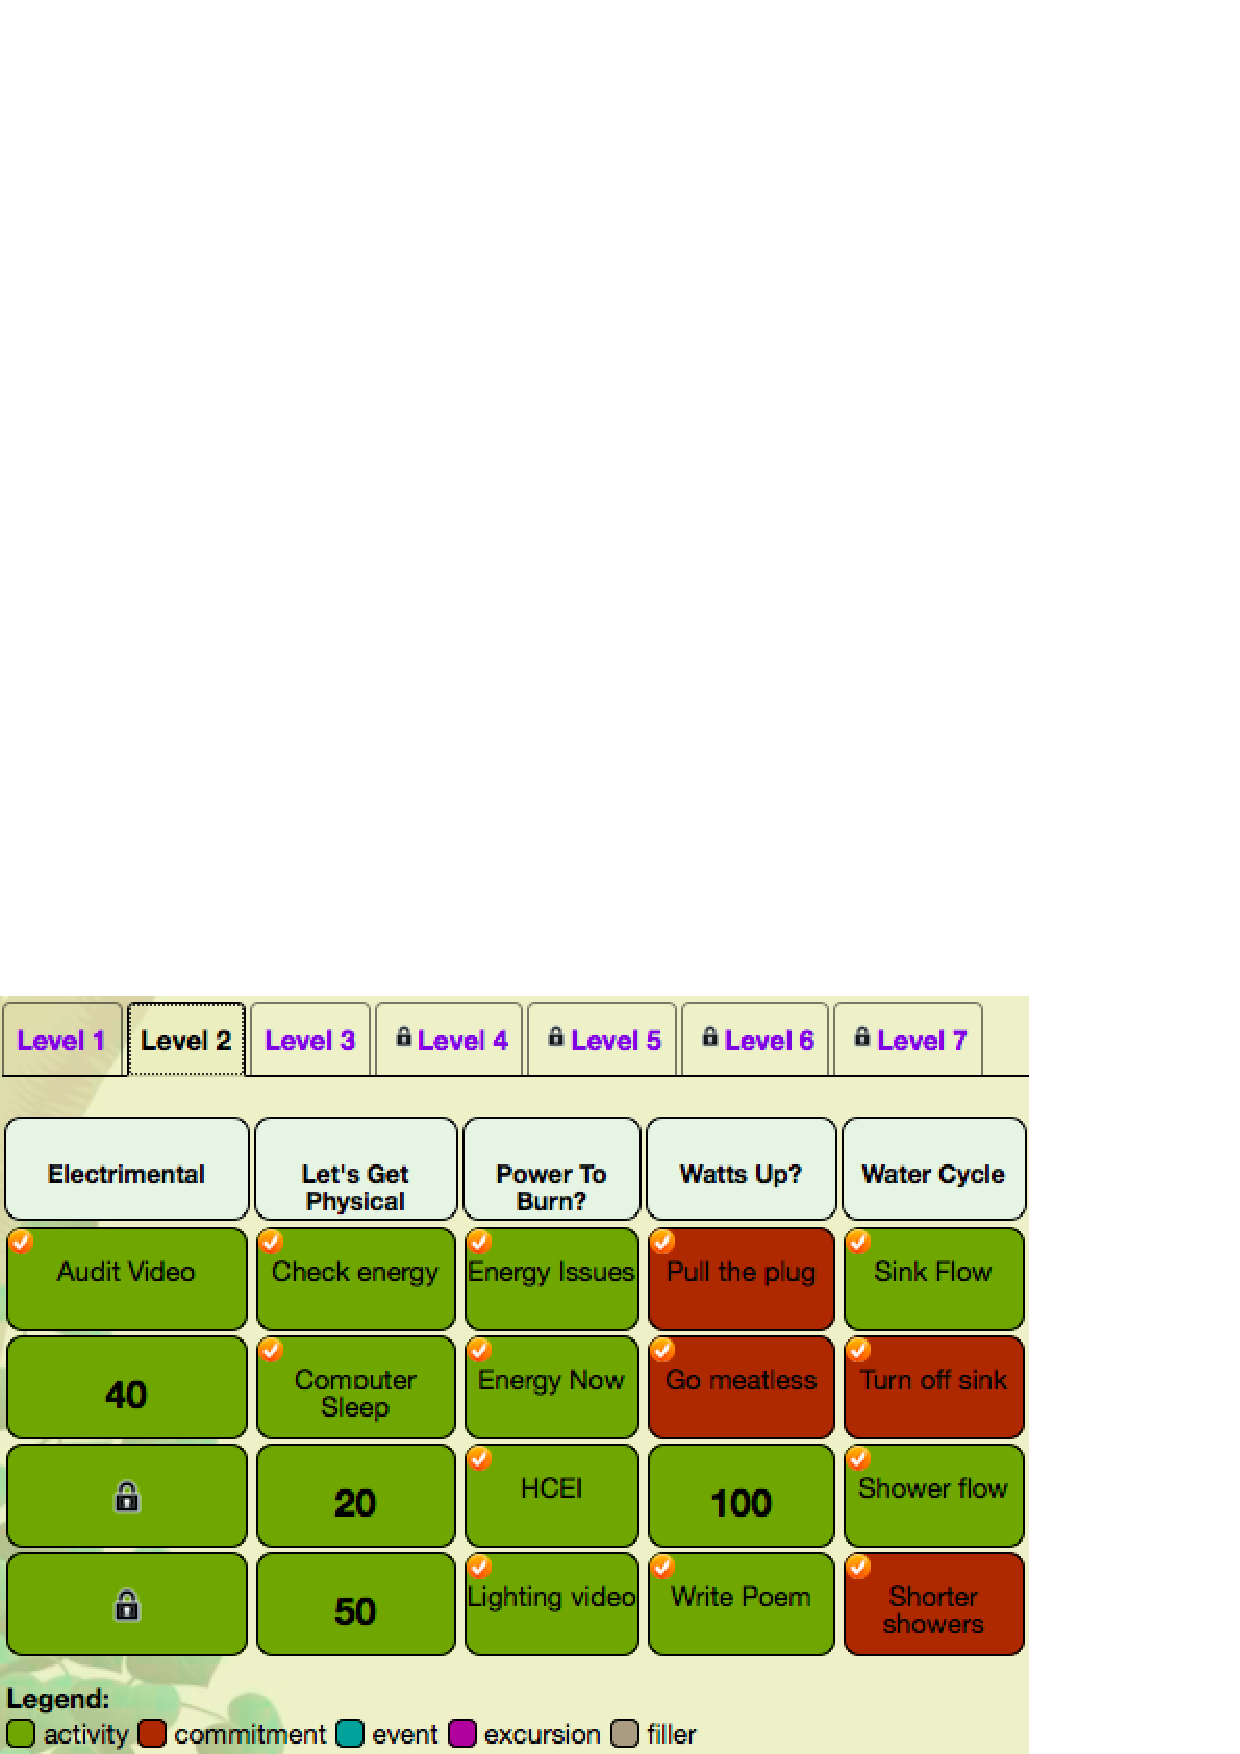
\includegraphics[width=0.7\textwidth]{smart-grid2}
	\caption{The level-based Smart Grid Game from Makahiki 2}
	\label{fig:smart-grid2}
\end{figure}

% Preliminary results?

As part of the 2012 UH Kukui Cup, Michelle Katchuck is investigating the motivations of residents regarding energy conservation as the subject of her Ph.D. dissertation.


\subsection{Makahiki 2 and Other 2012 Kukui Cups}
\label{sec:makahiki2}

After using Makahiki to support the 2011 UH Kukui Cup, we redesigned and reimplemented the Makahiki system to be more flexible and modular. Some of Makahiki 2's new features are:

\begin{itemize}
	\item The ability to customize all aspects of Makahiki to support Kukui Cup challenges tailored to the needs of an organization;
	\item The ability to support water use in addition to energy use, and enter the data manually in addition to the existing automated collection using WattDepot;
	\item Support for deploying Makahiki to a scalable cloud hosting provider (Heroku) to reduce cost and complexity for system administrators; and
	\item A new architecture intended to be easier for developers to modify and extend.
\end{itemize}

Two organizations ran their own Kukui Cup challenges in fall 2012 using Makahiki 2's new functionality: \Hawaii Pacific University (a private university in Honolulu), and the East-West Center (an education and research organization affiliated with the University of \Hawaii). These were the first deployments of the Kukui Cup outside of UHM, and provided new insight into the Kukui Cup, such as how to run a challenge without prizes, as the East-West Center did.


\subsection{Energy Literacy Questionnaire Improvements}

The energy literacy questionnaire I developed represents an initial attempt to create an instrument tailored to both \Hawaii and students living in a residence hall. It could be improved in several ways:

\begin{itemize}
	\item Further analysis of the questionnaire, examining: item difficulty, reliability (Cronbach's Alpha), and distractor analysis;
	\item Determining whether energy literacy results are stable across repeated measurements;
	\item Collaborating with other experts in the \Hawaii energy community to assess whether there are additional areas of energy knowledge the instrument should cover; and
	\item As the Kukui Cup expands beyond student residence halls, adapting the questionnaire to assess literacy in other populations.
\end{itemize}


\subsection{Additional Game Content}

Although the Kukui Cup now includes over 100 actions in its library of content, there are several additional areas that could be expanded. The Kukui Cup currently lacks an video explaining the important relationship between water and energy: many forms of energy generation require water, and use of water requires energy to pump, heat, cool, and treat. We also lack videos delving into \Hawaii's options for future energy use, and a Native Hawaiian perspective on energy issues.

One issue with the Kukui Cup is that the educational content is largely of interest only until its content has been assimilated. We do not anticipate that players would want to revisit most actions unless they were able to earn additional points. This limited engagement is in contrast to games that players enjoy playing over and over. Some serious games such as the protein folding game Foldit do manage to attract repeat players and meet their serious goals~\cite{Khatib2011}.

Beyond additional videos, the Kukui Cup could benefit from additional actions that are more interactive in the way people traditionally think of games. Developing a complete game requires much more effort than our current actions, but could potentially provide a much higher level of engagement among players. One option would be to partner with developers of educational energy games such as Energy City, a city simulation game where players pick must figure out how to supply the energy needs of a growing city while minimizing environmental impact~\cite{energy-city}. \autoref{fig:energy-city} shows a screenshot from Energy City.

\begin{figure}[htbp]
	\centering
	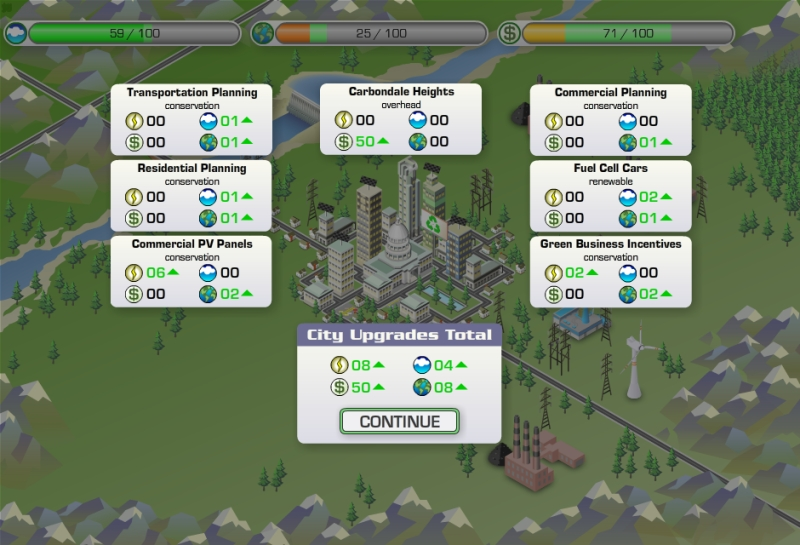
\includegraphics[width=\textwidth]{energy-city}
	\caption{The educational Energy City simulation game}
	\label{fig:energy-city}
\end{figure}


\subsection{Expansion Beyond Higher Education}

All of the Kukui Cup challenges held to date have been held in institutions of higher education (the participants in the East-West Center Kukui Cup were mostly students). While the student residence hall environment has been a useful setting for our initial research, the Kukui Cup could have greater impact if we expand to other settings.

One area we are actively exploring is deploying the Kukui Cup in the K-12 school environment. Schools have certain similarities to the student residence halls, in that the participants would be students, but many differences. In a K-12 environment, the Kukui Cup could be woven into existing curricula, rather than being an extra-curricular activity. The Kukui Cup action content would have to be redeveloped to be appropriate for the grade level being targeted, which is a substantial undertaking. Potentially energy data could be measured on a per building or per classroom basis, depending on the availability of smart metering infrastructure at the schools.

If the Kukui Cup is deployed at hundreds of schools in \Hawaii, we will need to make the solution easier to use for the challenge designers and managers, who will likely be teachers. Most of our effort in improving the user experience to date has been focused on the player, but with a large number of novice Kukui Cup challenge designers, we will need to switch our focus to improving the user experience both for the design of the challenge and for administering a challenge.

Beyond schools, the Kukui Cup could eventually be deployed to the general public. Several issues would need to be resolved before it could be deployed on such a wide scale:

\begin{itemize}
	\item The energy literacy content would have to be made sufficiently generic that it could apply to the wide range of potential participants.
	\item Makahiki would have to provide a way for participants to sign up for an account, something that is currently configured in advance by administrators.
	\item Energy data from homes would need to be imported into the system in some way. One promising option is the Green Button standard being promoted by the US Department of Energy, utilities, and companies interested in engaging customers with their electricity use~\cite{green-button}.
	\item The current manual approval of actions by administrators would need to be automated in some way, since manual approvals would not scale to many thousands of players.
\end{itemize}


\subsection{Refrigerator Usage}

Based on the prevalence of mini-refrigerator use (see \autoref{sec:appliance-count}), future iterations of the Kukui Cup should include programs designed specifically to address this issue. For example, when first moving into their rooms, residents could be strongly encouraged to share a refrigerator with their roommate. The impact of shared refrigerators on energy use would have to take into account the likelihood of purchasing larger refrigerators to accommodate shared usage. However, most mini-refrigerators have little insulation due to their smaller size, so a larger refrigerator will not necessarily use much more energy.
